\documentclass[a4paper]{article}

\usepackage{lgrind}
\usepackage{graphicx}
\usepackage{hyperref}

\author{Paul van der Walt\\\url{paul@denknerd.org}}
\date{\today}
\title{Parallel Algorithms: Eratosthenes' Sieve}

\begin{document}
\maketitle
\begin{abstract}
    In this report the findings are presented after benchmarking the Dutch
    supercomputer Huygens and a personal computer. The Sieve of Eratosthenes is
    then implemented in sequence and parallel (including a number of performance
    improvements), and tested on Huygens and a
    personal computer. 
\end{abstract}
\tableofcontents

\section{Introduction}

This report documents the use of BSP-style\cite{BSP} parallel programming to
find primes in parallel, using Eratosthenes' method. 

The so-called sieve of Eratosthenes is an old and unsophisticated method for
finding all primes up to a given number $N$, which lends itself quite nicely to
parallelisation. The idea is roughly as follows: start with the lowest known
prime $i$ (given: $i \leftarrow 2$ in the first iteration) and cross all
multiples of $i$ out of your list of potential primes, which starts off with all
natural numbers 1\ldots$N$. While $i$ is less than $N$, repeat. The next lowest
known prime is the smallest number which hasn't been crossed off the list yet.
More information about Eratosthenes' prime sieve can be found in Section
\ref{sec:sieve}. 

Secondly, we take a look at benchmarking BSP computers and the performance
measured when testing on Huygens\cite{sarahuygens}, the Dutch national
supercomputer, and on a recent MacBook. Specifically, the benchmark is aimed at
parallel computers, measuring not only computation speed, but also
synchronisation time and communication speed. 



\section{Prime Sieve}\label{sec:sieve}


\section{Benchmarks}

The two computers tested in this section, as already mentioned, are a recent
MacBook\footnote{Core2Duo 2.4Ghz with 4GB memory.} and Huygens, the national
supercomputer. Of course we didn't do the benchmark on all the nodes of Huygens,
as there are in the order of three thousand of them, but only on 1 and 2 nodes. 

The benchmark that has been done is the one included in BSPedupack which can be
found at \cite{edupack}, referred to as \texttt{bspbench.c}. The results are
presented in Figures \ref{fig:bench-huy-put-p2} to
\ref{fig:bench-laptop-get-p56}. In all these figures, the horizontal axis
represents the value of the $h$-relation, in other words, how many data words
are communicated in the communication superstep, and the vertical axis
represents the time (in flops) taken for the communication superstep.
Furthermore the well-known meanings of $r$, $g$ and $l$ hold, namely computation
rate, communication cost per data word in flops and sync time in flops,
respectively. 

\subsection{Original benchmark}
\begin{figure}[h]
    \begin{center}
        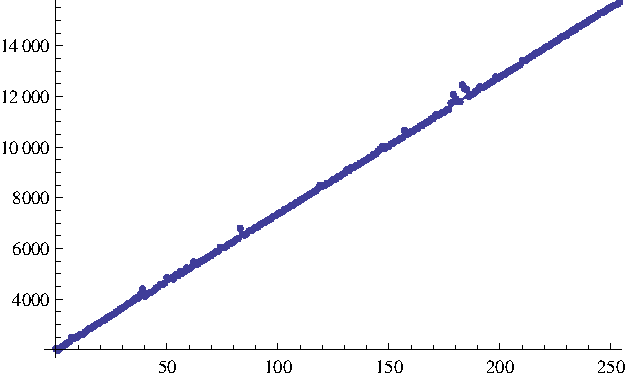
\includegraphics{img/bench-huy-put-p2.pdf}
    \end{center}
    \caption{Benchmark results on Huygens with $P$=2; the benchmark bottom line
    was $r=$ 194.357 Mflop/s, $g=$ 54.2, $l=$ 1986.4}
    \label{fig:bench-huy-put-p2}
\end{figure}

\begin{figure}[h]
    \begin{center}
        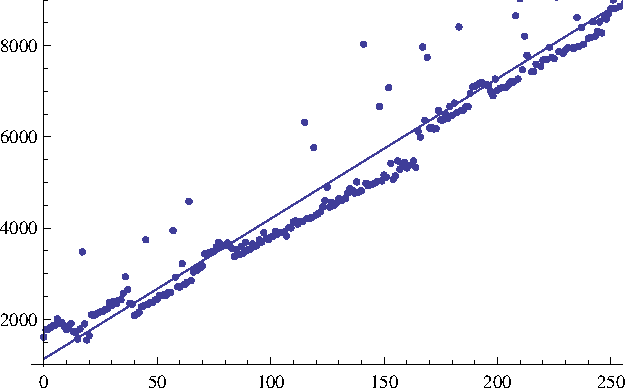
\includegraphics{img/bench-laptop-put.pdf}
    \end{center}
    \caption{Benchmark results on MacBook with $P$=2; bottom line was  $r=$
    399.853 Mflop/s, $g=$ 30.9, $l=$ 1112.4 }
    \label{fig:bench-laptop-put-p2}
\end{figure}

In figures \ref{fig:bench-huy-put-p2} and \ref{fig:bench-laptop-put-p2} we see
the results of running the plain benchmark on Huygens and the laptop.
Interestingly enough, the laptop seems to perform better than Huygens in all
respects. The only reason we can give for this is that the shared cores on
Huygens are a lot more overworked than the laptop when it is doing nothing else
other than running the benchmark. In a sense this is therefore an unfair
comparison.

Note that on Huygens we used 1 node, which means the communication would
probably be cheaper than if we were to do the same benchmark, but distribute it
over 2 nodes, so the communication has to leave the node as opposed to being
local, as it would have been in Figure  \ref{fig:bench-huy-put-p2}. 

We see predictable and expected linear behaviour on Huygens, but the laptop
results are a
lot more noisy. We attribute this to the fact that other processes such as the
graphical user interface are running which generate unpredictable performance
hits. These observations also hold on the get-versions of these 2 tests.

\begin{figure}[h]
    \begin{center}
        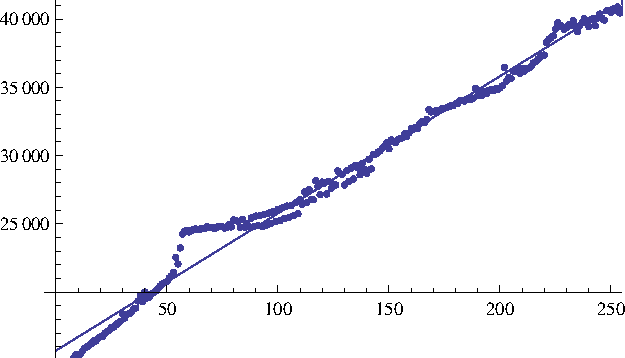
\includegraphics{img/bench-huy-put-p2-dist.pdf}
    \end{center}
    \caption{The same test as in Figure \ref{fig:bench-huy-put-p2}, but then
    instead of 2 processes on one node, we tried 2 processes on 2 nodes. The
    bottom line becomes $r=$ 195.648 Mflop/s, $g=$ 100.2, $l=$ 15770.4}
    \label{fig:bench-huy-put-p2-dist}
\end{figure}

The results shown in Figure \ref{fig:bench-huy-put-p2-dist} are when we select 2
distinct nodes on Huygens. We indeed see a marked increase in communication cost
$g$ and synchronisation cost $l$. As we would expect, the computational rate $r$
is basically unaffected by this change, as the work needing to be done locally
is the same as before. 

Since here we are forcing network communication, the performance becomes more
interesting to analyse. Where the local version (Figure
\ref{fig:bench-huy-put-p2}) has a very straight performance ``curve'', we now
observe a peak and some waviness. The waviness is attributed to other network
communication outside of our control which will affect the speed with which our
packets reach their destination; the peak is possibly the point at which the
underlying layer decides to switch to another, more high-volume, communication
scheme. The latter point is, however, guesswork, without knowing more about our
platform. 

\subsection{Changing to \texttt{get}s}
Now we change puts into gets in the benchmark algorithm. The hypothesis is that
getting is more expensive than putting, since a put is passive with respect to
the receiver, whereas when getting both processors have to work. See figures
\ref{fig:bench-huy-get-p2} to \ref{fig:bench-huy-get-p2-dist}. 

\begin{figure}[h]
    \begin{center}
        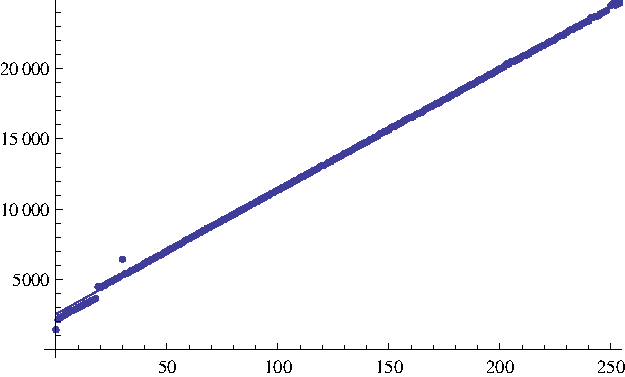
\includegraphics{img/bench-huy-get-p2.pdf}
    \end{center}
    \caption{Having changed \texttt{put}s into \texttt{get}s we measure again on
    Huygens with $P=2$. Bottom line: $r=$ 191.062 Mflop/s, $g=$ 87.2, $l=$ 2574.6}
    \label{fig:bench-huy-get-p2}
\end{figure}

\begin{figure}[h]
    \begin{center}
        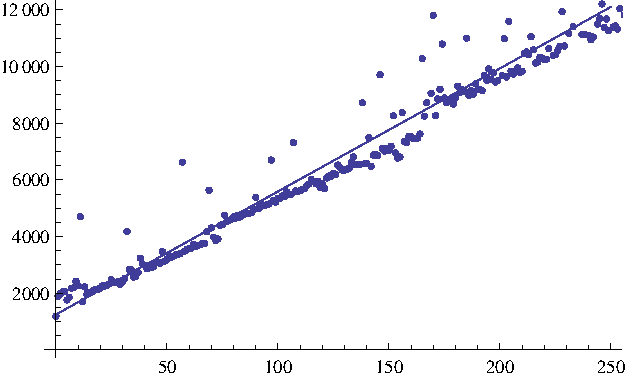
\includegraphics{img/bench-laptop-get.pdf}
    \end{center}
    \caption{MacBook with $P=2$. Bottom line: $r=$ 389.348 Mflop/s, $g=$ 43.5, $l=$ 1240.1}
    \label{fig:bench-laptop-get-p2}
\end{figure}

Comparing \ref{fig:bench-huy-get-p2} and \ref{fig:bench-laptop-get-p2} to the
corresponding figures in the previous section, we indeed see a marked increase
in communication cost (note: not in synchronisation cost) on Huygens. Surprisingly enough, on the laptop, this
increase is not so great on the laptop. We expect and observe the
synchronisation time to be comparable with puts and gets, since this change
shouldn't affect the synchronisation steps. 

\begin{figure}[h]
    \begin{center}
        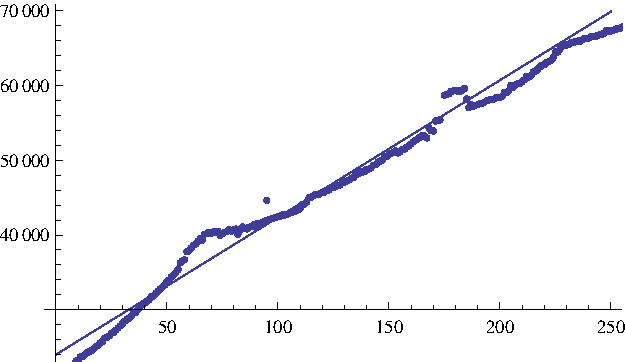
\includegraphics{img/bench-huy-get-p2-dist.pdf}
    \end{center}
    \caption{The same test as in Figure \ref{fig:bench-huy-get-p2}, but then
    instead of 2 processes on one node, we tried 2 processes on 2 nodes. The
    bottom line becomes $r=$ 194.498 Mflop/s, $g=$ 182.3, $l=$ 24222.0}
    \label{fig:bench-huy-get-p2-dist}
\end{figure}

Once again, we try forcing the benchmark to run on 2 distinct nodes on Huygens
(see Figure \ref{fig:bench-huy-get-p2-dist}). Again the computation rate $r$ is
the same, communication cost $g$ is significantly increased, but in this case,
also $l$ suffers, increasing by nearly a factor of 2. We cannot give an
explanation for this, and attribute it to incidental load on the shared node
being used. Note that this is plausible seeing the entire benchmark runs in
about 20 seconds, which will never give a very accurate picture of a computers
average performance. 

We also see not 1, but at least 2 discernible peaks in the curve. Once again the
conjecture is that the communication schemes used switch at these points. 

As a last effort at producing more interesting results, we run the benchmark on
the laptop with $P=56$. This isn't done on Huygens since it will be a waste of
resources and will probably have to wait a long time in the queue. See Figure
\ref{fig:bench-laptop-get-p56}. The results here speak for themselves: the
computation rate $r$ is still independent of the configuration, but the
communication cost and specifically synchronisation time skyrocket. The reasons
for this are obvious: namely, communication becomes more costly when the
underlying BSP layer has to manage more and more processors, and the
synchronisation cost is hypothesised to be $\omega(n)$ (i.e. at least linearly increasing in
the number of processors used, $N$). 

\begin{figure}[h]
    \begin{center}
        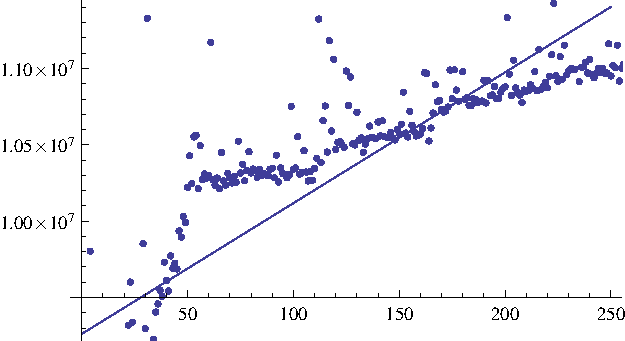
\includegraphics{img/bench-laptop-get-p56.pdf}
    \end{center}
    \caption{Test on the MacBook with $P=56$, using \texttt{get}s. Bottom line
    now becomes $r=$ 445.799 Mflop/s, $g=$ 4201.9, $l=$ 10037639.0}
    \label{fig:bench-laptop-get-p56}
\end{figure}

Interestingly we also see a sharp increase in communication time before $h=56$,
where after that point the time levels out to become linear. This is logical,
since before $P=56$, not all processors are being communicated with, so the
communication superstep takes much longer each time an extra processor is talked
to. After all the processors have been communicated with (i.e. $h>56$) BSP is
smart enough to bundle communication to a given processor, so that the
communication time increases linearly in $h$. 



\appendix
\section{Sequential sieve code}\label{app:seq}

\lgrindfile{../seq/sieve.lg}

\section{Parallel sieve code}\label{app:par}

\lgrindfile{../par/bspsieve.lg}


\begin{thebibliography}{99}
    \bibitem[BSP]{BSP} \url{http://www.bsp-worldwide.org}, homepage of the BSP
        association. 
    \bibitem[SHuy]{sarahuygens}
        \url{https://subtrac.sara.nl/userdoc/wiki/huygens/description},
        information page on the Huygens supercomputer. 
    \bibitem[BSPep]{edupack}
        \url{http://www.staff.science.uu.nl/~bisse101/Software/software.html}, homepage of BSPedupack, an education set of sample code for the
        BSP library. 
\end{thebibliography}

\end{document}
